\subsection{Model-Iteration-Based Offline Style Transfer}

As previously mentioned, although pixel-iteration-based style transfer methods have the ability to perform arbitrary style transfers, their low efficiency prevent them from being widely used in real-life scenarios, especially when dealing with tasks involving a large number of images. This drawback is particularly evident in such cases. To improve the efficiency of neural style transfer, researchers have developed fast-style transfer methods that trade off either the quality of style transfer or the number of transferable styles. These methods are referred to as model-iteration-based style transfer.

Generally, the primary approach to achieving model-iteration-based style transfer is to shift the time required during inference to the training phase. Specifically, this is typically done by training a specific style transfer network, which stores style information in the form of parameters within the network. When confronted with different styles, the network can quickly retrieve the corresponding parameters, thereby enabling fast style transfer.

From a historical perspective, model-iteration-based style transfer can be divided into two stages: the first stage involves a single model generating a single style, and the second involves a single model generating multiple styles. To help readers accurately classify the methods used in the literature, this paper provides detailed descriptions of these two categories: if a style transfer method takes a content image as input and the network can quickly convert it into a specific stylized image, the method can be classified as Per Model Per Style transfer. On the other hand, if a style transfer method takes a content image and the encoded representation of the desired final style as input, and the network can quickly convert it into a stylized image corresponding to the style code, the method can be classified as Per Model Multi Style transfer. 

\subsubsection{Per Model Per Style}

\textbf{Using feedforward networks to achieve Per Model Per Style.} Johnson et al.\citep{22johnson2016perceptual} and Ulyanov et al.\citep{23ulyanov2016texture} were the first to publish work on real-time style transfer. Independently, in 2016, they both proposed methods for real-time style transfer using feedforward neural networks. The main idea was to train a feedforward neural network that encodes style information in the network's parameters, allowing the generation of stylized images without the need for multiple iterations of optimization on a noise image. Specifically, the following feedforward neural network needs to be trained: 
\begin{equation}
    \begin{aligned}
        \theta^* &= \arg\min L_{total}\left(I_c,I_s,g_\theta*(I_c)\right),\\
        I^*&=g_\theta*(I_c),
    \end{aligned}
\end{equation}
where $\theta^*$ represents the optimal parameters that minimize the total loss function $L_{total}$.

The total loss function $L_{total}\left(I_c,I_s,g_\theta*(I_c)\right)$ evaluates the quality of the style transfer. This function has three inputs: the content image $I_c$, the style image $I_s$, and the stylized image $g_\theta*(I_c)$. It produces a single output, $I^*$, which is the final stylized image. The goal of this function is to find the parameters $\theta^*$ that minimize $L_{total}$. These parameters are used to transform the content image $l_c$ into the final stylized image $I^*$.
\begin{figure}[!htbp]%% placement specifier
    %% Use \includegraphics command to insert graphic files. Place graphics files in 
    %% working directory.
    \centering%% For centre alignment of image.
    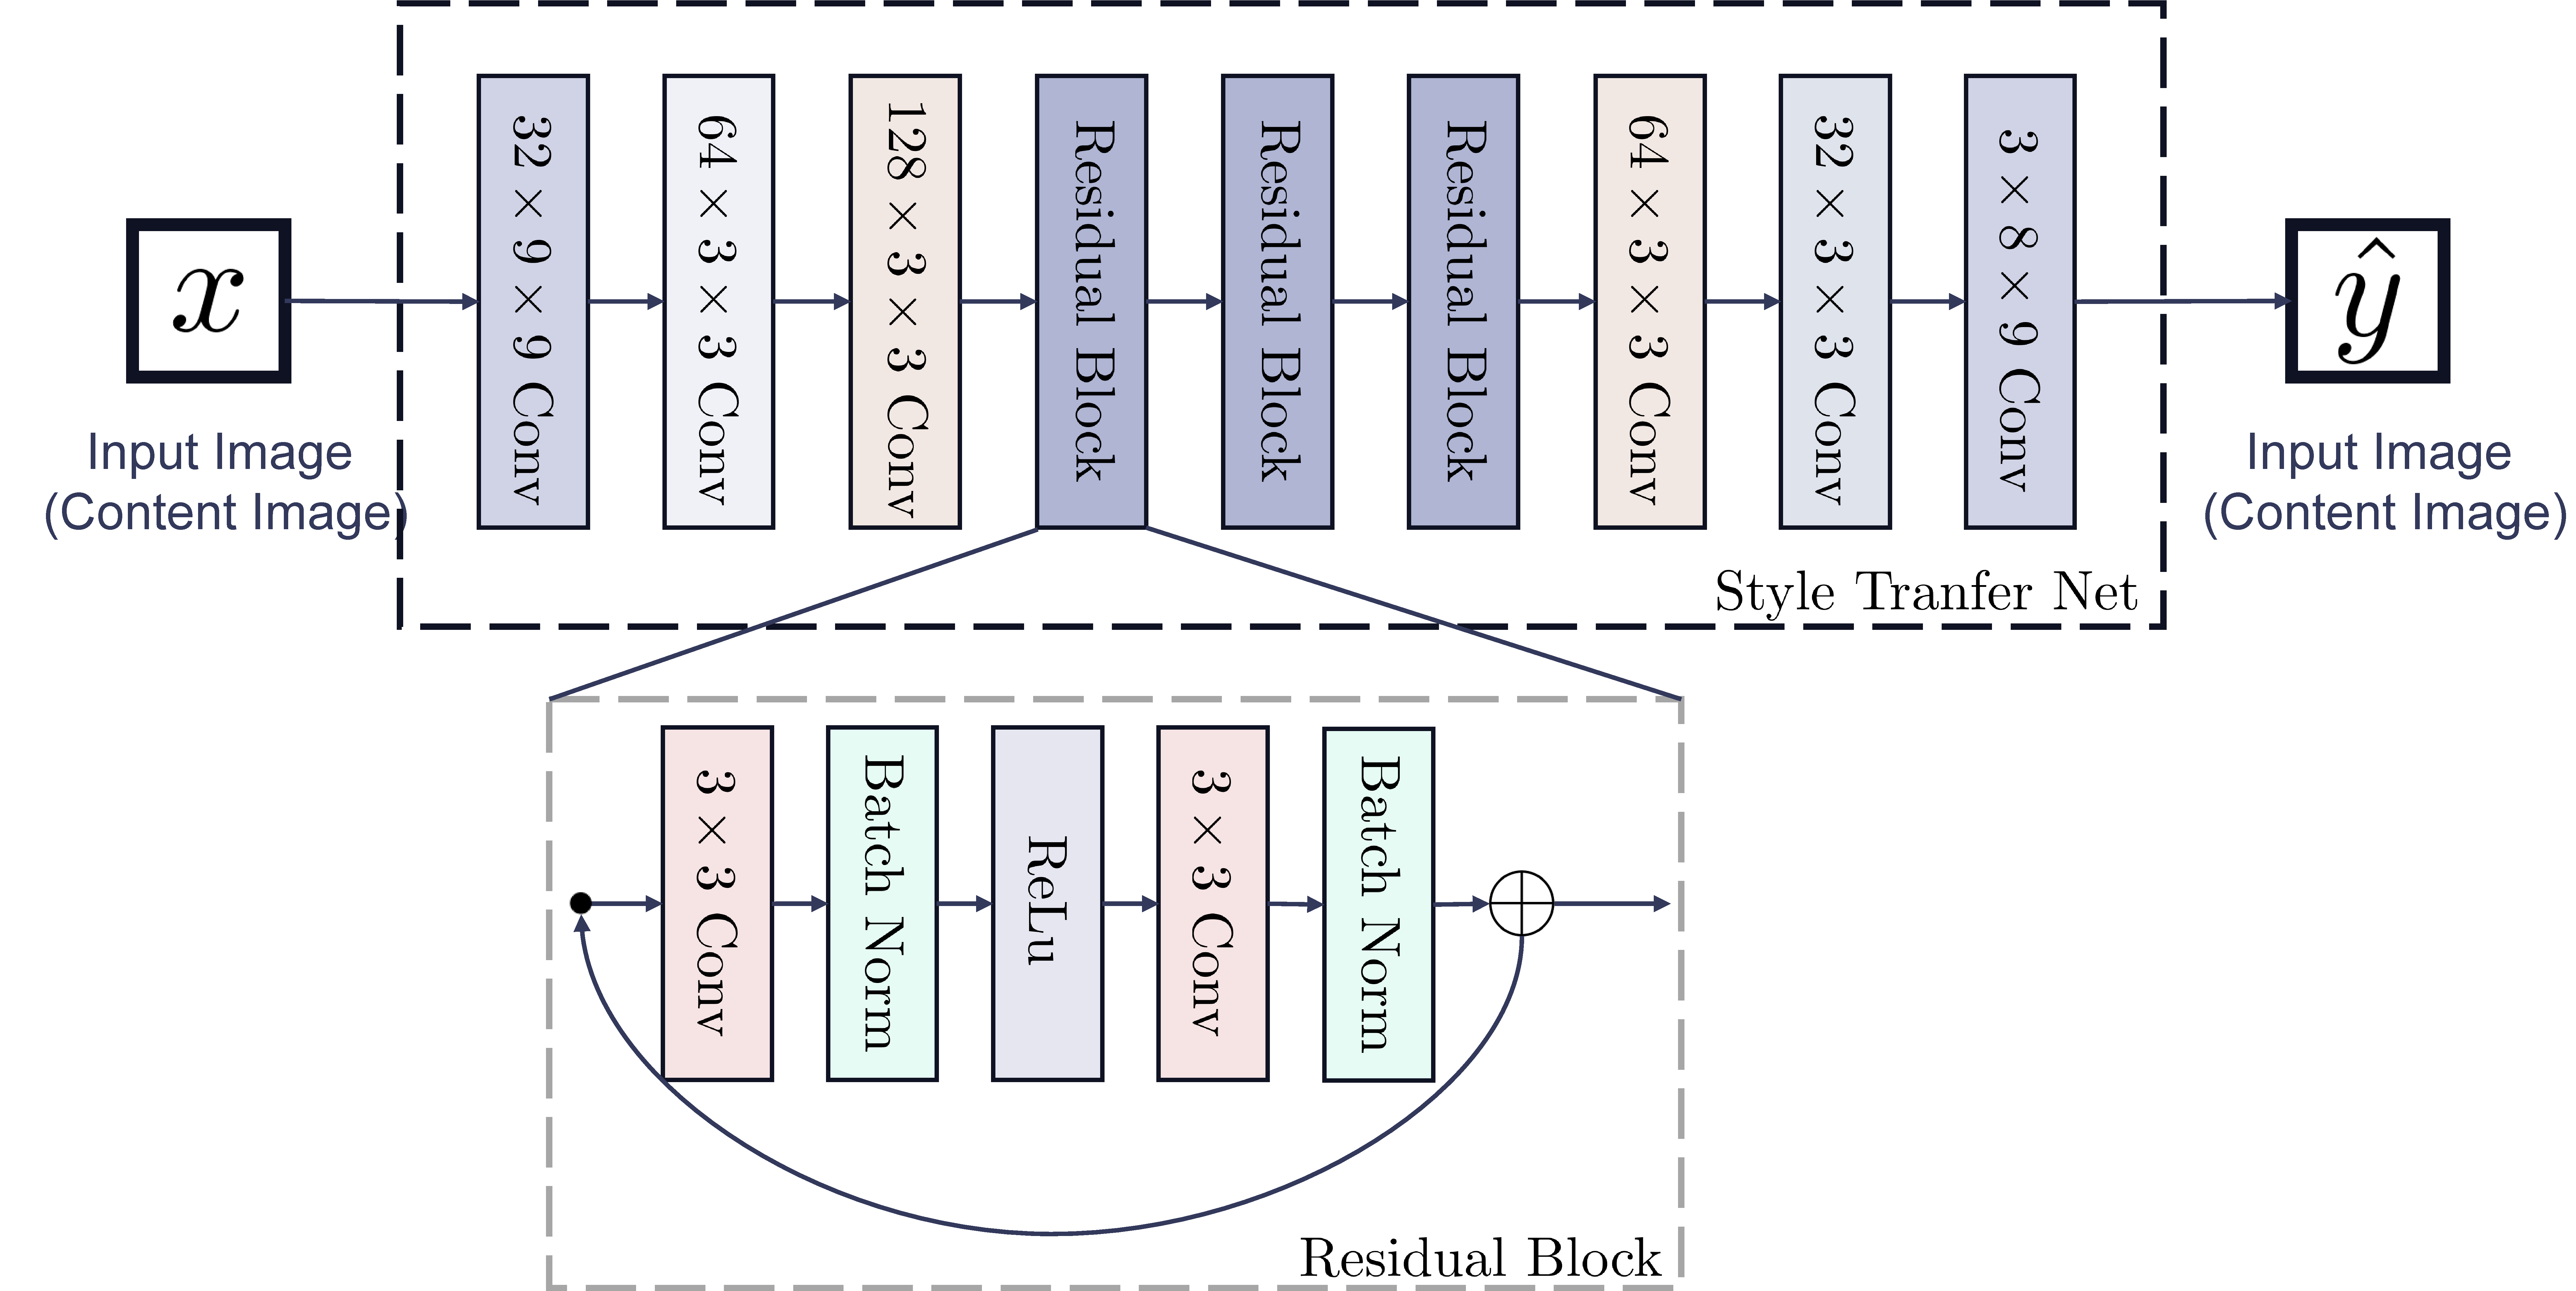
\includegraphics[width=0.95\textwidth]{fig/Figure_3_Johnson_et_al's_Network_Architecture_[22].pdf}
    %% Use \caption command for figure caption and label.
    \caption{Johnson et al.'s Network Architecture \citep{22johnson2016perceptual}}\label{fig4_Johnson}
\end{figure}

Although Johnson et al. and Ulyanov et al. proposed this method simultaneously, there are differences in their network structures. Johnson\citep{22johnson2016perceptual} et al. built upon the method by Radford et al.\citep{34radford2015unsupervised}, adding residual blocks and step-wise convolution, and introduced an Instance Normalization (IN) layer to accelerate the network's convergence, as shown in Figure \ref{fig4_Johnson}.


On the other hand, Ulyanov et al.\citep{23ulyanov2016texture} used a multi-scale structure as the generative network (as shown in Figure \ref{fig5_Ulyanov}), with an objectiveKwo function similar to that of Gatys et al.\citep{02gatys2016image} Both Johnson et al. and Ulyanov et al. based their methods on feedforward generative networks, achieving real-time style transfer. Compared to the method by Gatys et al.\citep{02gatys2016image}, the speed of style transfer was improved by two orders of magnitude.

\begin{figure}[!htbp]%% placement specifier
    %% Use \includegraphics command to insert graphic files. Place graphics files in 
    %% working directory.
    \centering%% For centre alignment of image.
    \includegraphics[width=0.95\textwidth]{fig/Figure_4_Ulyanov_et_al_'s_Network_Architecture_[23].pdf}
    %% Use \caption command for figure caption and label.
    \caption{Ulyanov et al.'s Network Architecture\citep{23ulyanov2016texture}}\label{fig5_Ulyanov}
\end{figure}

However, since both methods during training largely follow the approach proposed by Gatys et al., they encounter similar issues in migration effects, such as unsatisfactory results in image detail and structural consistency.

\textbf{Using Markov Random Fields for Per Model Per Style.}\quad The use of Markov Random Fields can also enhance the speed of style transfer. Li and Wand et al.\citep{35li2016precomputed} improved their previous work\citep{33li2016combining} by obtaining a Markov feedforward network through adversarial training (Figure 5), thereby addressing the efficiency problem. In principle, this method is similar to their earlier non-parametric style transfer approach based on image patches described in\citep{33li2016combining}. This improvement allows them to achieve better results in object structure consistency, thereby preserving the fine details of the original image more effectively. However, some shortcomings of the original methods remain, such as poor performance when the matching between local patches and style patches is not precise.

\begin{figure}[!htbp]%% placement specifier
    %% Use \includegraphics command to insert graphic files. Place graphics files in 
    %% working directory.
    \centering%% For centre alignment of image.
    \includegraphics[width=0.95\textwidth]{fig/Figure_5_Li_et_al_'s_Network_Architecture_[35].pdf}
    %% Use \caption command for figure caption and label.
    \caption{Li et al.'s Network Architecture\citep{35li2016precomputed}}\label{fig6_Ulyanov}
\end{figure}

\textbf{Using Generative Adversarial Networks for Per Model Per Style.}\quad Using Generative Adversarial Networks (GANs) for style transfer represents another approach to Per Model Per Style transfer.

GANs were introduced by Goodfellow et al. in 2014\citep{36goodfellow2020generative}. This model consists of a generator network and a discriminator network that engage in adversarial training. During training, the discriminator network is first trained: given a set of data, the discriminator evaluates whether each data item belongs to the target domain. Then the discriminator is optimized based on the discrepancy between the true values and the network's judgments until it can accurately classify data items in the test set. Subsequently, the generator is trained to produce data, which is then assessed by the discriminator to determine if it belongs to the target domain. The generator adjusts itself based on the feedback from the discriminator. The generator and discriminator continuously compete to balance each other, leading to the training of the network and achieving a similarity in distribution between the generated data and the real data. The loss function for GANs is as follows:

\begin{equation}
    \label{GAN_loss}
    V(D,G)=\mathbb{E}_{x\sim p_{\text{data}}(x)}\left[\log D(x)\right]+\mathbb{E}_{z\sim p_{\text{z}}(z)}\left[\log \left(1-D(G(z))\right)\right]
\end{equation}

In this context, $G$ and $D$ represent the generator network and the discriminator network, respectively. $p_{\text{data}}(x)$ denotes the distribution of the data $x$, $p_{\text{z}}(z)$ denotes the distribution of noise images, $D(x)$ represents the probability that $x$ belongs to the real data rather than the data generated by the generator $p_g$, and $G(z)$ denotes the generator's output for the noise image $z$. $E$ represents the expectation. The discriminator is trained to maximize the probability that it can distinguish between images from the dataset and those generated by $G$. The generator's training aims to minimize $\log \left(1-D(G(z))\right)$, where $1-D(G(z))$ represents the probability that the discriminator believes the generated image does not belong to the real data set. Minimizing this function deceives the discriminator into thinking that the generated data comes from the real data set. The excellent network structure of GANs makes them suitable for style transfer tasks.

\begin{figure}[!htbp]%% placement specifier
    %% Use \includegraphics command to insert graphic files. Place graphics files in 
    %% working directory.
    \centering%% For centre alignment of image.
    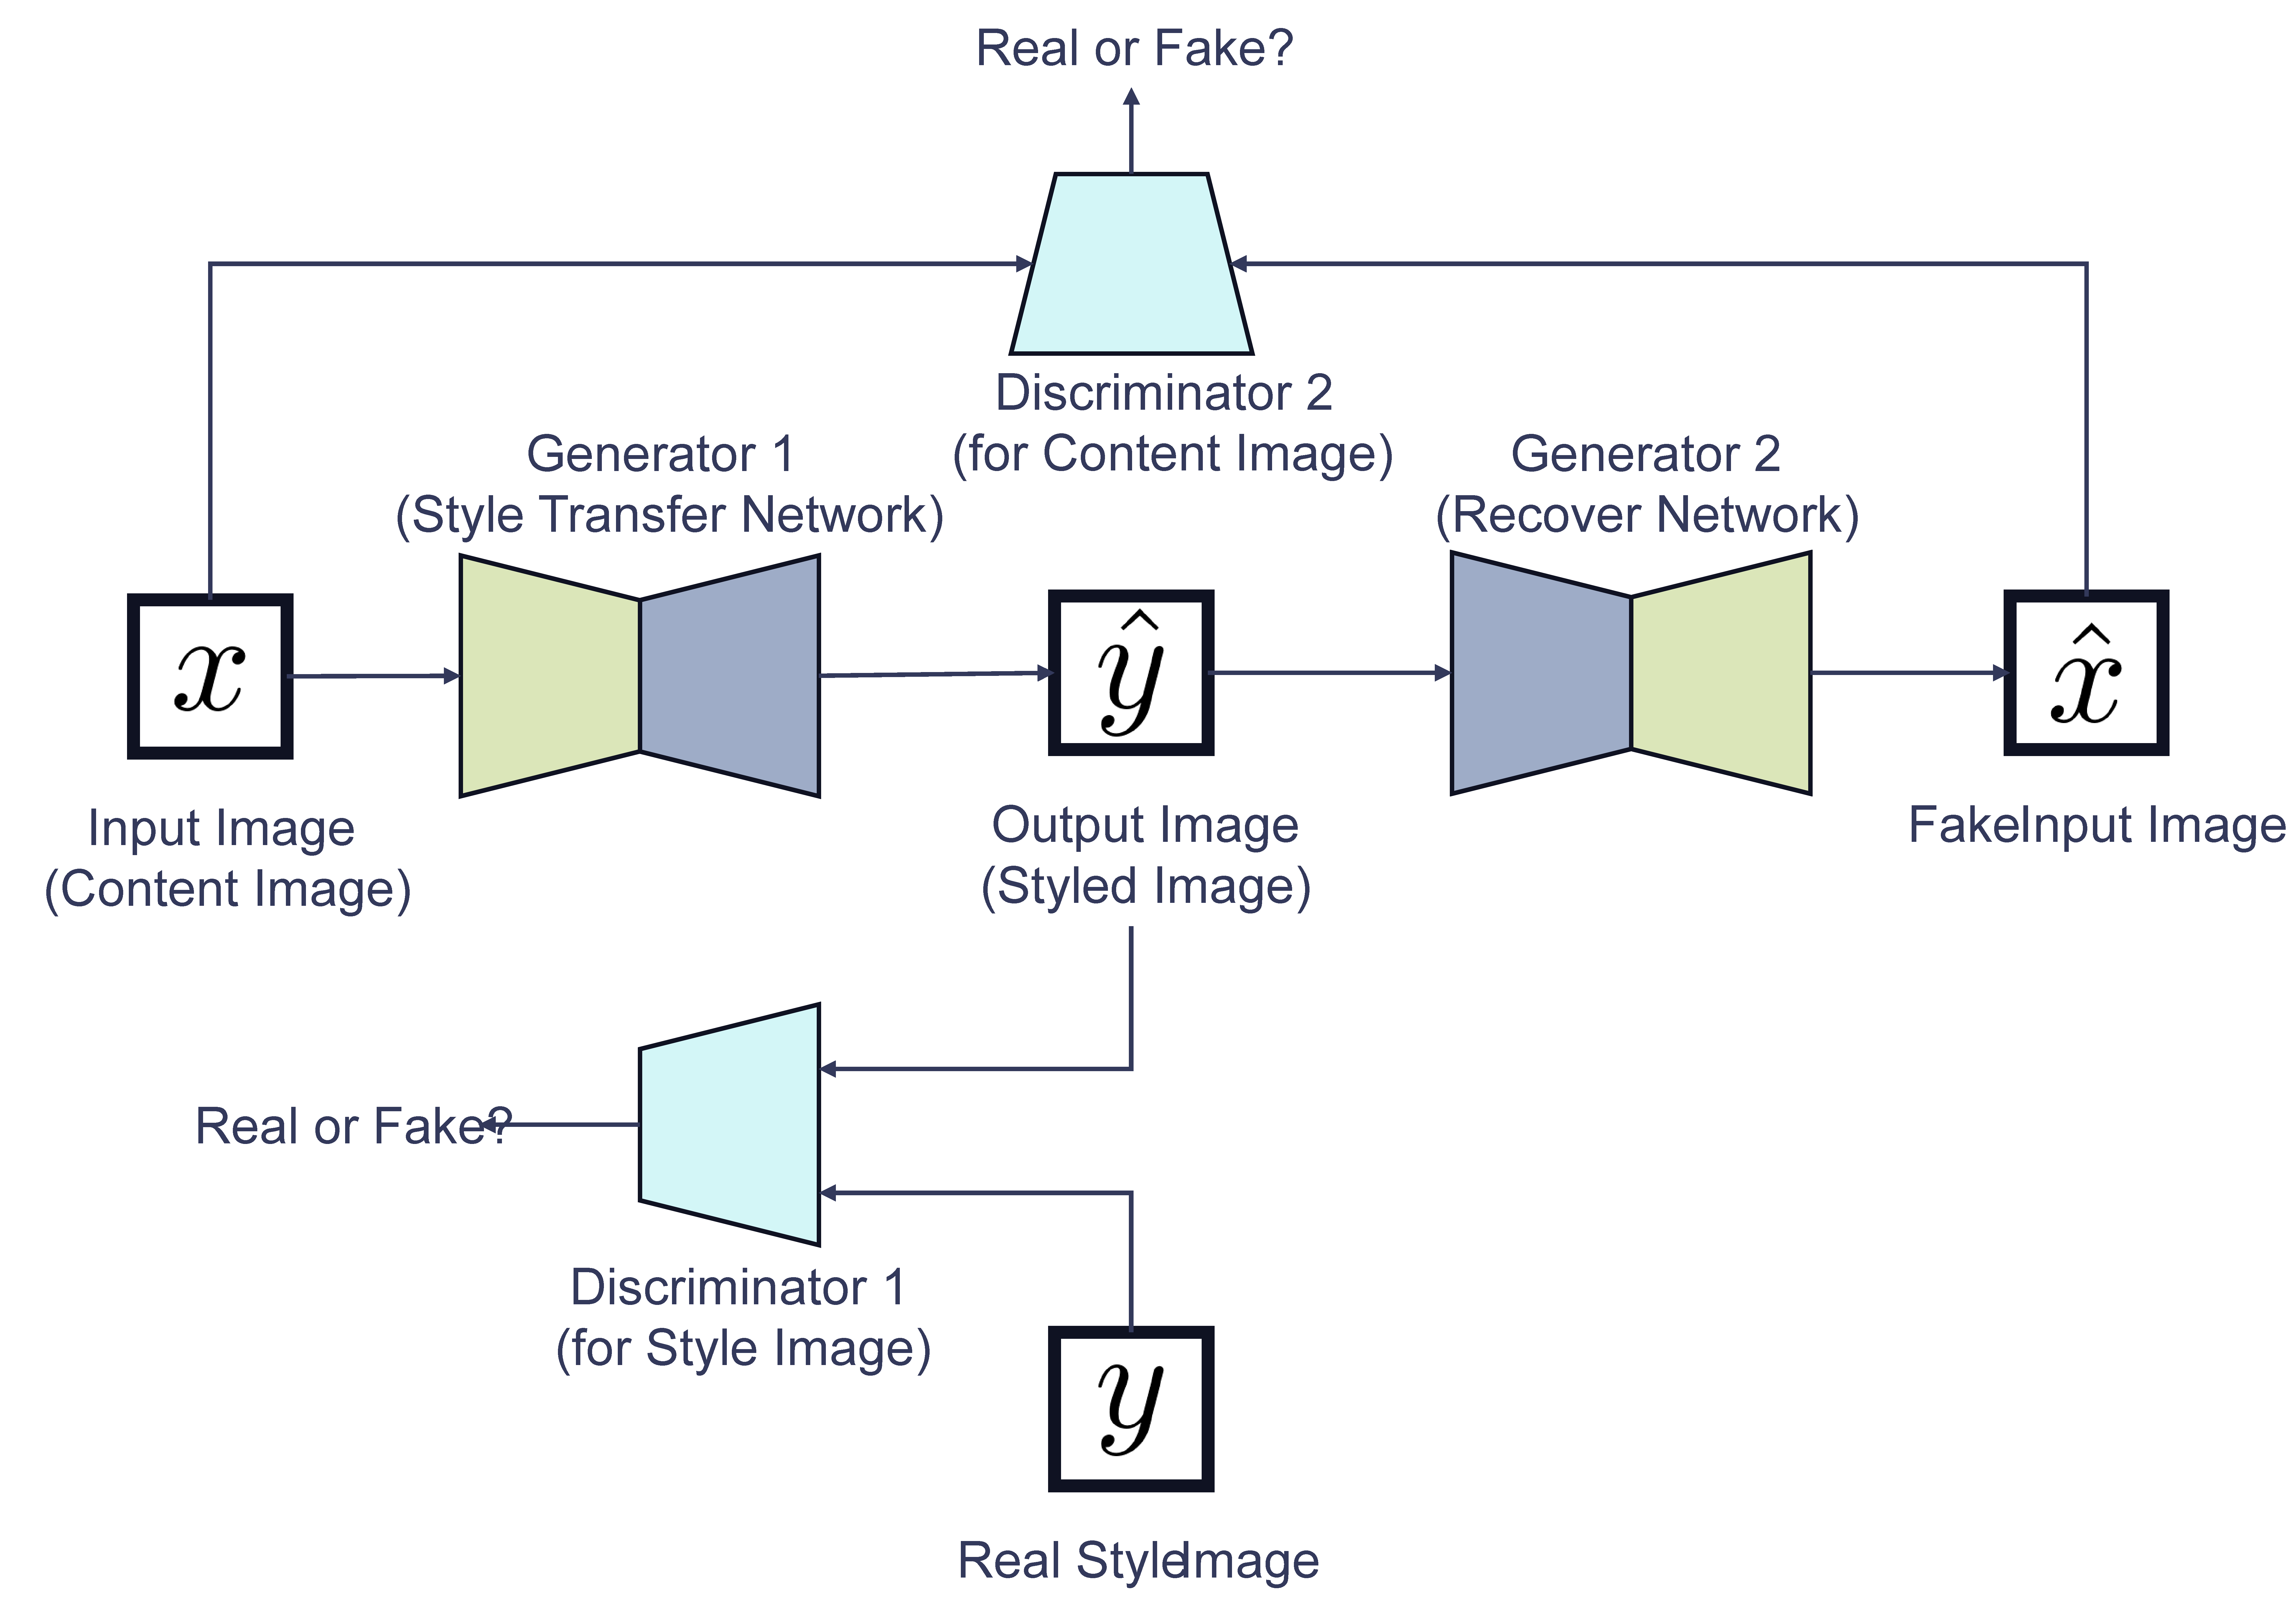
\includegraphics[width=0.95\textwidth]{fig/Figure_6_Workflow_of_CycleGAN_[38].pdf}
    %% Use \caption command for figure caption and label.
    \caption{Workflow of CycleGAN \citep{37zhu2017unpaired}}\label{fig7_Zhu}
\end{figure}

However, GANs face several issues and drawbacks when applied to real-time style transfer. Firstly, training GANs is often challenging and can be unstable, leading to problems such as mode collapse. Secondly, the loss function of GAN models does not include hyperparameters like $\alpha$ and $\beta$ from Gatys et al.’s\citep{02gatys2016image} loss function, making it difficult to control the similarity between the generated image and the content or style images. Therefore, precise control in style transfer tasks is challenging. While GANs can be used for style transfer tasks, they are not specifically designed for these tasks.

Zhu et al.\citep{37zhu2017unpaired} modified GANs\citep{38goodfellow2014generative} to better adapt to real-time style transfer tasks. In their work\citep{37zhu2017unpaired}, they proposed CycleGAN, which achieves unsupervised Per Model Per Style style transfer. CycleGAN's uniqueness lies in its introduction of "cycle consistency loss," which ensures bidirectional transformations by simultaneously training two generators and two discriminators, thus preserving information through conversions from one domain to another and back. Similar to GANs, CycleGAN\citep{37zhu2017unpaired}'s generator maps images from one domain to another, while the discriminator tries to distinguish between generated and real images (Figure \ref{fig7_Zhu}).



One of the advantages of CycleGAN is its ability to handle unpaired data, enabling unsupervised learning. This method can learn how to perform cross-domain image translation without requiring explicit pairings for each sample during training. However, CycleGAN also has some notable drawbacks in the field of style transfer. The images it generates can sometimes appear blurrier or distorted than real images. Additionally, improper selection of hyperparameters may reduce the stability of the training process or result in poor image quality.

StyleGAN\citep{19karras2019style} is another outstanding achievement in using GANs for style transfer, particularly known for its portrait editing capabilities, which can generate portraits with specific features and high realism. StyleGAN controls various details and the overall style of the generated image by adjusting the "style" parameters in the input latent space. The core innovation of StyleGAN is the introduction of a new style transfer mechanism, which allows for the separate control of image content and style at different levels, thereby improving the diversity and controllability of generated images while maintaining image quality. The advantages of StyleGAN include its ability to generate high-resolution, high-quality images and provide powerful image editing capabilities through style control. It performs exceptionally well in generating faces and other complex images. However, the training process is resource-intensive and time-consuming, requiring significant computational resources. Additionally, the generated images may sometimes contain unpredictable artifacts, necessitating further optimization to improve stability and reliability.

Men et al.\citep{46Men_2022_CVPR} focused on portrait style transfer, aiming to transform portrait photographs into anime-style avatars. They observed that when using CycleGAN for style transfer involving significant geometric deformations, it is challenging to generate high-quality transfer results while preserving the correct structure. To address this issue, the authors proposed an unsupervised cartoon image generation method based on a Gated Cycle Mapping Network (GCMN). The core of this approach is the introduction of a Gated Style Encoder (Egs), which generates category-specific style codes through domain and group-specific style layers and injects these codes into the generator to achieve precise style control.

Traditional CycleGAN models enforce bidirectional mapping, requiring multiple generators, which perform poorly when dealing with complex geometric structural changes, especially in the conversion from portraits to anime, where high-quality outcomes cannot be assured. To mitigate this limitation, Men et al. designed a gated style encoder that combines gated mapping units (GMUs) with domain-specific and group-specific layers to generate category-specific style codes, thereby achieving precise control over the transformation process. The domain-specific layers distinguish whether the image originates from the photo domain or the cartoon domain, while the group-specific layers further differentiate between portraits and scenes, ensuring the rationality and accuracy of the style transfer. Additionally, the authors introduced an Adaptive Instance Normalization (AdaIN) mechanism to inject the style codes into the generator via a multi-layer perceptron (MLP), dynamically modulating the stylistic expression within the generated results.

In contrast to traditional multi-generator or multi-encoder methods, the Gated Cycle Mapping Network requires only a single generator to handle image translation tasks in all directions, significantly simplifying the model architecture. Experimental results demonstrated that the gated style encoder not only enhanced the quality of the generated cartoon images but also allowed for flexible migration according to user-specified style requirements, thus achieving higher controllability. With these improvements, the authors' model surpassed existing state-of-the-art methods in terms of visual effects and style control and also exhibited superior performance in video synthesis tasks.Per Model Per Style transfer can mitigate the primary drawbacks of long transfer time and low efficiency of pixel-iteration-based style transfer by shifting the time required for the transfer phase to the training phase. However, the trade-off is that it can only transfer a specific, single style. If multiple styles are to be transferred using this method, corresponding network training is required for each style, resulting in a large number of parameters. In such cases, the large number of parameters makes it difficult to deploy on devices with limited resources (e.g., smartwatches), thus necessitating a balance between the number of styles and the performance constraints.

\subsubsection{Per Model Per Style}

Although the Per Model Per Style methods addressed the issue of real-time stylization and improved the efficiency of style transfer, each model can only correspond to a specific style. Transferring to a new style requires significant time for training a new model, and it is challenging to apply these models to the devices with limited resources. To address this, the networks capable of transferring multiple styles while maintaining the ability to perform fast transfers, known as Per Model Multi Style networks, are developed. One of the main approaches to achieving multi-style transfer is to bind a specific style to a small portion of the network parameters to reduce redundant parameters and combine this with the addition of necessary parameters that reflect style differences in the networks.

Dumoulin et al.\citep{39dumoulin2016learned} were the first to bind specific styles to parameters within the network, thereby achieving Per Model Multi Style transfer. In reducing redundant parameters, they noted that certain parts of the computation in the transfer of different styles are similar or identical, as many artistic styles with different names share similar or identical brushstrokes (for example, Impressionist paintings have similar brushstrokes, differing mainly in the colors used). It seems wasteful to treat these paintings with similar brushstrokes as entirely different styles. Traditional one-to-one style transfer models overlooked this, leading to unnecessary time wastage during the training phase when transferring to a new style.
In their experiments, Dumoulin et al.\citep{39dumoulin2016learned} found that scaling or transforming the normalized parameters is sufficient to adapt to a particular style. For a convolutional neural network, this finding implies that the parameters of all convolutional kernels can be adjusted to facilitate the transfer of different styles. Specifically, style transfer can be achieved by simply adjusting certain parameters of the convolutional kernels after normalization. In implementation, Dumoulin et al.\citep{39dumoulin2016learned} built upon the method of Ulyanov et al. \citep{23ulyanov2016texture}, applying an affine transformation after instance normalization to complete the transfer of different styles. This process is referred to as Conditional Instance Normalization (CIN), which can be represented by the following formula:

\begin{equation}
    \label{IN}
    \text{CIN}\left(\mathcal{F}(I_c,s)\right) = \gamma^s\left(\frac{\mathcal{F}(I_c)-\mu(\mathcal{F}(I_c))}{\sigma(\mathcal{F}(I_c))}\right)+\beta^s
\end{equation}
The input to the formula consists of the content image $I_c$ and the style index $s$, with $F(x)$ representing the feature map of image x, and $\mu(x)$ and $\sigma(x)$ representing the mean and standard deviation of the image, respectively. This method achieved the transfer of different styles by scaling or transforming the parameters $\gamma^s$ and $\beta^s$, meaning that each style s can be realized by adjusting the parameters of the affine transformation.

The advantage of this approach is that by using affine transformations on parameters of similar styles, Dumoulin et al. were able to reduce redundant parameters, significantly lowering the number of required parameters compared to Per Model Per Style methods when generating the same number of styles. However, when dealing with images with significant style differences, it is still necessary to retrain the network to obtain the corresponding style parameters and adjustment methods. Therefore, as the number of transferable styles increases, the network parameters in this method also increase.

Chen et al.\citep{40chen2017stylebank} achieved parameter simplification through a different method. Unlike Dumoulin et al.\citep{39dumoulin2016learned}, who used similar parameters to represent similar styles, Chen et al. \citep{40chen2017stylebank} considered content image processing, proposing that the parts of the network that process content information could be the same. This led to the concept of decoupling the content processing module and the style processing module within the network. By using this decoupling approach, with independent network modules learning the content and style information of an image, the network becomes more flexible in handling style transfer tasks. This method employs mid-level convolutional filters (referred to as the "StyleBank" layer in\citep{40chen2017stylebank}, as shown in Figure \ref{fig8_Chen}) specifically designed to learn different styles. The "StyleBank" layer contains multiple sets of parameters, with each set associated with a specific style.

\begin{figure}[!htbp]%% placement specifier
    %% Use \includegraphics command to insert graphic files. Place graphics files in 
    %% working directory.
    \centering%% For centre alignment of image.
    \includegraphics[width=0.95\textwidth]{fig/Figure_7_Network_Architecture_of_Chen_et_al_[41].pdf}
    %% Use \caption command for figure caption and label.
    \caption{Network Architecture of Chen et al.\citep{40chen2017stylebank}}\label{fig8_Chen}
\end{figure}

The other parts of the network, aside from the "StyleBank" layer, are used to learn content information. Since the content processing module handles different styles in the same way, different styled images can use the same content processing module, thereby improving the network's efficiency in processing various styles. When implementing multi-style transfer, only incremental training is needed. Specifically, when a new style needs to be added, the part of the network responsible for learning content information can be fixed, and only the "StyleBank" layer for the new style is trained. This approach allows the network to effectively learn new styles without affecting the existing learned ones. In the StyleBank, one or more sets of convolutional kernels represent a specific style. By placing different sets of convolutional kernels into the neural network, it can perform style transfers for different styles, providing good scalability.

Although this approach allows a single network to transfer multiple styles and optimizes the number of parameters in the network, challenges still remain. In terms of parameters, if the method attempts to transfer multiple styles, the number of parameters will gradually increase with the number of transferable styles, making it impossible for this approach to handle arbitrary style transfers. Regarding the quality of generated images, due to the partial parameter sharing, the transfer quality might not reach the excellent results of style transfer methods based on model iteration.
